\section{Introduction}
In order to sucessfully comission the Vera C. Rubin Observatory and begin the Legacy Survey of Space and Time (LSST) we need to be able to perform astrometric and photometric calibrations of individual visits. 
This calibration will be done in the rubin science pipelines by comparing instrumental fluxes of stars to a reference catalog.
To meet the science requirements for relative photometric precision (OSS-REQ-0387) the rms of repeated measurements of unresloved sources must be, at a miniumum, less than 8 mmag (12 mmag) for gri-band (uzy-band) observations. 
Additionally, the requirements for the astrometric quality of data are defined in OSS-REQ-038 are such that the rms on the distance between pairs of sources must be less than 10 milli-arcseconds, with an error on the accuracy of less than 50 mas in any axis. 
To achieve these goals we need a reference catalog with the following features:

\begin{itemize}
    \item The catalog must cover any location we will want to point the telescope. This includes the full sky with declination < 30 deg, althogh we have generated an all-sky catalog. 
    \item There must be flux estimates in all bandpasses, ugrizy for LSSTCam and grizy for LATISS. 
    \item The number density of un-saturated high-signal to noise sources must be high enough to calibrate a single LSSTCam CCD. 
    The size of a detector on the sky is X.X which is approximately the same size as an Nside=256 healpixel. 
    \item High precision measurements of the positions of unresolved sources. 
    This is achived by using Gaia Dr3 as the basis for the objects in our catalog with full position and proper motion measurements included. 
    
\end{itemize}

Previous catalogs such as ATLAS-RC2 provide the all-sky coverage, but are not sufficently deep to provide the required source density. 
PS1 provides the depth in \emph{grizy}-bands but not the *u*-band or the all-sky coverage. 
Therefore, we have developed \emph{the\_monster}, a combination of reference catalogs similar to ATLAS-RC2 but with the bandpass coverage and depth required to enable LSST. 

\textbf{Note:} In this document we use \emph{source} to describe the bandpass a measurment is currently in and \emph{target} to describe the bandpass we would like to transform a measurement into. 

\section{Summary of creation of \textit{the\_monster}}
The creation of the \textit{the\_monster} can roughly speaking be broken into two components, the \textit{grizy}-bands and the *u*-band. 


\subsection{\textit{grizy-bands}}
\begin{enumerate}
    \item For each input reference catalog, we retrieve a version containing only high-quality stellar sources.
    \item Subsequently, all input catalogs are converted into the LSST refcat format (htm7), see Catalog Conversion section.
    \item Our reference catalog, \textit{the\_monster}, uses DES bandpasses internally for \textit{grizy}-bands. The next step is to convert all measured fluxes to the DES system. This is done by fitting a cubic spline to the ratio of source flux and target flux as a function of color. Additionally, for PS1, we found a magnitude-dependent offset that has been fit as well. The Colorterms section describes these fits in more detail.
    \item With the external reference catalogs in hand, as well as colorterms for each measurement, we next create versions of each refcat that have been matched to \textit{Gaia\_DR3} sources, further selected to only include isolated sources (no neighbors within 1"), and transformed to the DES bandpass.
    \item Finally, we assemble the monster by reading in each transformed htm shard and adding measurements for each \textit{Gaia\_DR3} (a rank order of preference is used when multiple refcats have measurements of the same source) to the\_monster catalog. We add flux measurements for the DES-bandpasses as well as any target bandpasses for the\_monster catalog. In version one of the\_monster, \textit{the\_monster\_20240904}, LATISS fluxes and synthLSST fluxes are included as well.
\end{enumerate}

\subsection{u-band}
For the \textit{u}-band, the creation process is similar with a few notable exceptions:
\begin{itemize}
    \item The internal system is SDSS \textit{u}-band.
    \item Gaiaxp tied to SDSS \textit{u}-band as described in the section.
    \item We use a stellar locus regression-based method to transform DES \textit{g}-band fluxes and \textit{g-r} colors into SDSS \textit{u}-band measurements.
\end{itemize}

The rest of this technote is organized as follows: each of the steps in monster creation is described in more detail. Then, we show all diagnostic plots for each input refcat.

\section{Input Data}
Here we describe the input catalogs used for the creation of The Monster. For each catalog, we include the origin, any cuts applied, and summary plots of the spatial distributions. The photometric catalogs used in this process are (in order of priority):
\begin{itemize}
    \item DES Y6 Calibration Stars
    \item Gaia XP Synthetic Magnitudes
    \item PS1
    \item SkyMapper
    \item VST
\end{itemize}

For \textit{u}-band we use:
\begin{itemize}
    \item SDSS Standard Stars
    \item Gaia XP Synthetic Magnitudes
    \item Stellar Locus Regression-based magnitudes
\end{itemize}

\section{Catalog conversion}
To convert the catalogs into LSST format, we follow the instructions on \href{https://pipelines.lsst.io/modules/lsst.meas.algorithms/creating-a-reference-catalog.html}{how to generate an LSST reference catalog} using the \href{https://pipelines.lsst.io/modules/lsst.meas.algorithms/tasks/lsst.meas.algorithms.ConvertReferenceCatalogTask.html#lsst-task-lsst-meas-algorithms-convertreferencecatalog-convertreferencecatalogtask}{ConvertReferenceCatalogTask}. Each refcat requires its own configurations, which can be found in the \href{https://github.com/lsst-dm/the_monster/tree/main/configs}{configs folder of the\_monster github repo}. Here we include an example configuration used for the \hyperref[des-y6-calibration-stars]{DES Y6 Calibration Stars}.

\section{Color Transformations}
\subsection{To DES Bandpasses}
\begin{figure}
    \centering
    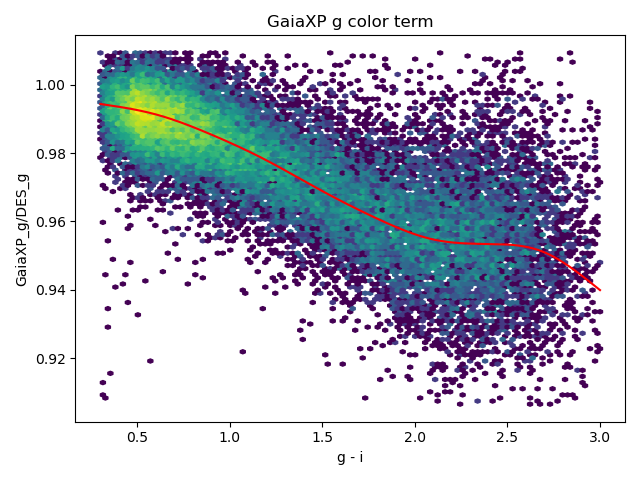
\includegraphics[width=\linewidth]{./figures/color_terms/GaiaXP_to_DES_band_g_color_term.png}
    \caption{Ratio of fluxes between GaiaXP synthetic photometry and DES for the \textit{g}-band as a function of \textit{g-i} color. The red line shows the cubic spline that defines our color transformation.}
    \label{xp-to-des-g-colorterm}
\end{figure}

\begin{figure}
    \centering
    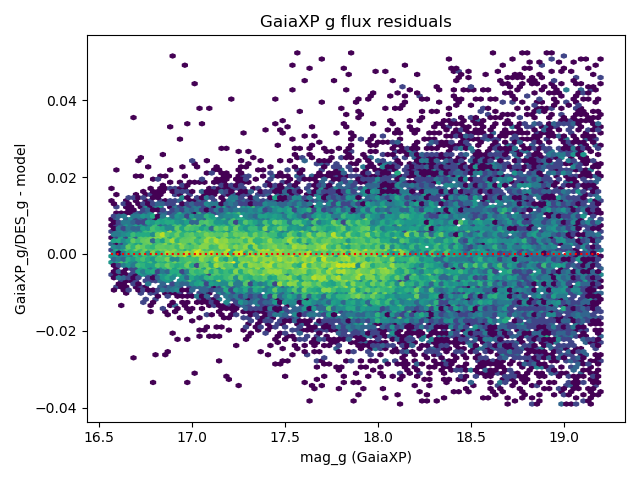
\includegraphics[width=\linewidth]{./figures/color_terms/GaiaXP_to_DES_band_g_flux_residuals.png}
    \caption{Residuals between GaiaXP synthetic photometry transformed to DES and DES as a function of magnitude.}
    \label{xp-to-des-g-residual}
\end{figure}

\subsection{To Synthetic LSST Bandpasses}
\subsection{To LATISS Bandpasses}
\subsection{To SDSS \textit{u}-band}

\section{Assembly of the\_monster v1}
\subsection{Source Count Maps}
\begin{figure}
    \centering
    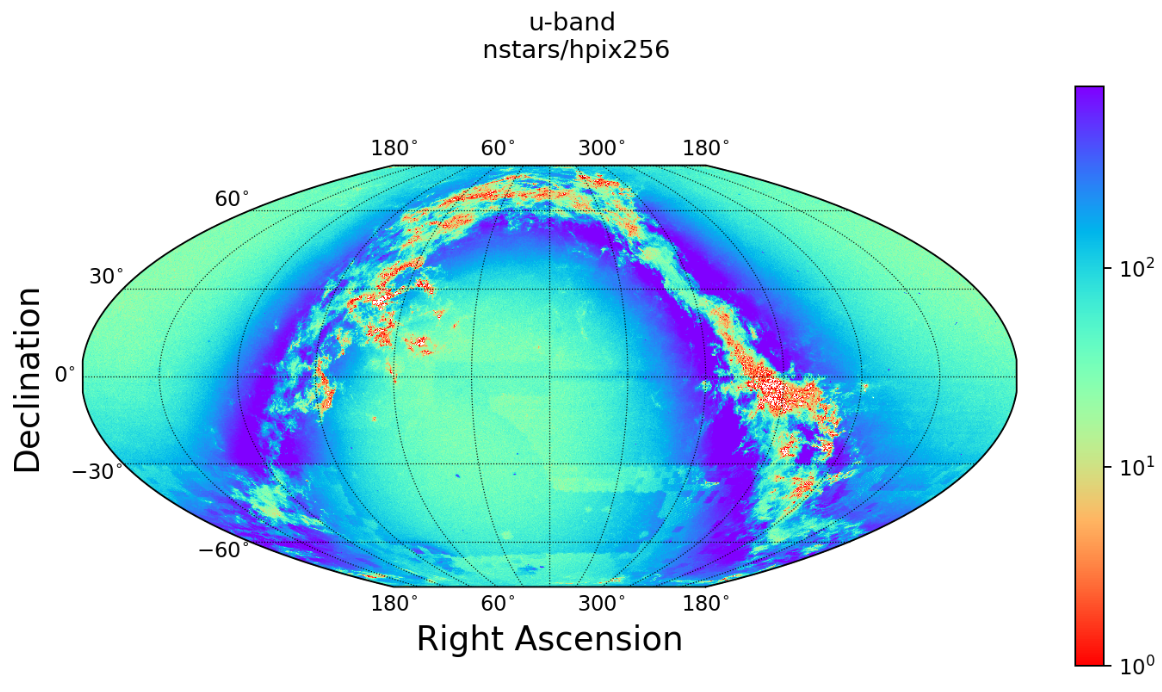
\includegraphics[width=\linewidth]{./figures/source_density_maps/u-band/u-band-counts-full.png}
    \caption{Map showing the number of sources with a \textit{u}-band measurement per \texttt{nside}=256 healpixel.}
    \label{source-counts-u}
\end{figure}

\subsection{Source Flag Maps}
\begin{figure}
    \centering
    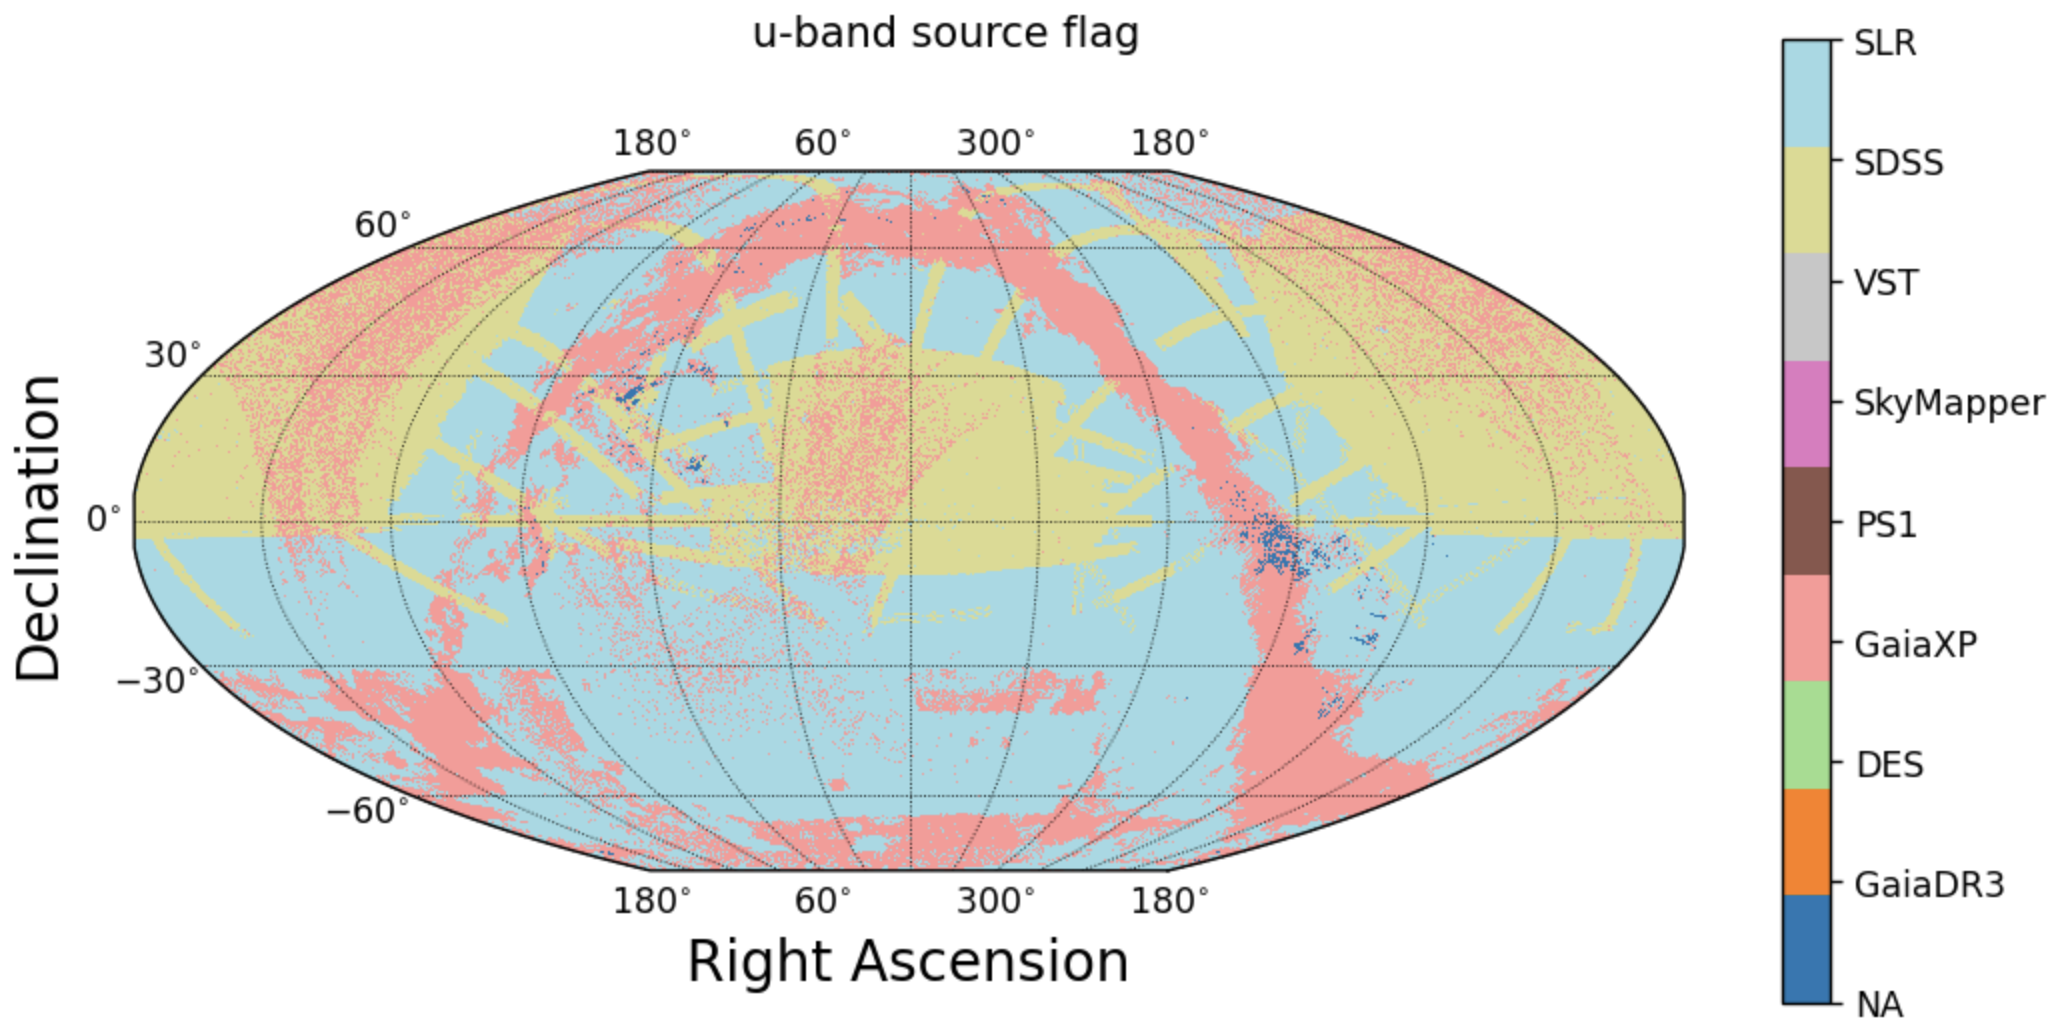
\includegraphics[width=\linewidth]{./figures/source_survey_maps/u-band_source.png}
    \caption{Map showing the median source of objects at each point in the sky for the \textit{u} band.}
    \label{source-flag-u}
\end{figure}

\section{Detailed Descriptions}
In the following subsections, we describe the external photometric catalogs used in the creation of the\_monster.

\subsection{DES Y6 Calibration Stars}
Data is described in \href{https://arxiv.org/abs/2305.01695}{Rykoff et al 2023}. Briefly, this is a catalog of calibrated reference stars generated by the Forward Calibration Method (FGCM) pipeline (arXiv:1706.01542) as part of the FGCM photometric calibration of the full Dark Energy Survey (DES) 6-Year data set (Y6). This catalog provides DES \textit{grizY} magnitudes for 17 million stars with \textit{i}-band magnitudes mostly in the range 16 < \textit{i} < 21, spread over the full DES footprint covering 5000 square degrees over the Southern Galactic Cap at galactic latitudes \textit{b} < -20 degrees (plus a few outlying fields disconnected from the main survey footprint). These stars are calibrated to a uniformity of better than 1.8 milli-mag (0.18\%) RMS over the survey area. The absolute calibration of the catalog is computed with reference to the STISNIC.007 spectrum of the Hubble Space Telescope CalSpec standard star C26202; including systematic errors, the absolute flux system is known at the approximately 1\% level. These stars provide a useful reference catalog for calibrating \textit{grizY}-band or \textit{grizY}-like band photometry in the Southern Hemisphere, particularly for observations within the DES footprint.

The data was retrieved from \url{https://data.darkenergysurvey.org/public_calib/DES_6yr_CalibStarCat/Y6A1_FGCM_V3_3_1_PSF_ALL_STARS.fits} on May 2nd, 2023.

Data page is at \url{https://des.ncsa.illinois.edu/releases/other}

\subsection{Color transformations}
The DES bandpasses act as the internal bandpasses for \textit{the\_monster} and 

\subsection{Gaia XP Synthetic Magnitudes}
This catalog contains synthetic fluxes/magnitudes for stars in the following passbands:
PS1std-grizy, PS1-grizy, DECam-grizY, SDSSstd-ugriz (and non-std), SkyMapper-u2uvgriz

Photometry was generated from Gaia DR3 XPSpectra \cite{https://arxiv.org/abs/2206.06215}. 

This was done using GaiaXPy \cite{https://github.com/gaia-dpci/GaiaXPy/cd}.

\subsection{PS1}
\url{/sdf/group/rubin/datasets/refcats/htm/v1/ps1_pv3_3pi_20170110/README.txt}

This reference catalog, intended for use with the LSST Science Pipelines \cite{https://pipelines.lsst.io} was constructed from the "3pi.pv3.20160422" DVO catalog of Processing Version 3 of the Pan-STARRS1 3pi survey, released to the Pan-STARRS1 Science Consortium. Following the public release of this data in December 2016 \cite{http://panstarrs.stsci.edu}, you may distribute this catalog freely.

This format of the catalog contains 2,990,470,528 point sources at Dec > -30 deg to i ~ 22.5 mag, and has a total size of 423 GB. 

Relevant papers for information and citation include:
\begin{itemize}
    \item Chambers et al., "The Pan-STARRS1 Surveys", 2016arXiv161205560C
    \item Magnier et al., "The Pan-STARRS Data Processing System", 2016arXiv161205240M
    \item Waters et al., "Pan-STARRS Pixel Processing: Detrending, Warping, Stacking", 2016arXiv161205245W
    \item Magnier et al., "Pan-STARRS Pixel Analysis: Source Detection and Characterization", 2016arXiv161205244M
    \item Magnier et al., "Pan-STARRS Photometric and Astrometric Calibration", 2016arXiv161205242M
    \item Flewelling et al., "The Pan-STARRS1 Database and Data Products", 2016arXiv161205243F
    \item Tonry et al., "The Pan-STARRS1 Photometric System", 2012ApJ...750...99T
    \item Schlafly et al., "Photometric Calibration of the First 1.5 Years of the Pan-STARRS1 Survey", 2012ApJ...756..158S
\end{itemize}

\subsection{SkyMapper}

\subsection{VST}

VST ATLAS DR4 downloaded from ESO archive.

Documentation can be found at: \url{http://www.eso.org/rm/api/v1/public/releaseDescriptions/90}

Skim to healpixels was done with the following criteria:
\begin{verbatim}
sel = (dat["MERGEDCLASS"] == -1)  # stars
sel &= (dat["PRIORSEC"] == 0)     # unique source 
sel &= (dat["PRIMARY_SOURCE"] == 1) # primary source 
sel &= (dat["UERRBITS"] < 0)      # no u-band processing flags
\end{verbatim}

\subsection{GAIA DR3 - The Astrometric Reference}
Original data: \url{https://www.cosmos.esa.int/web/gaia/dr3}

The full Gaia DR3 catalog in indexed HTM format. This is the first LSST refcat to contain the full coordinate covariance.

Magnitude range: $\sim$3 - 21 (G magnitude)



% \section*{Methods}

% \subsection*{grizy-bands}
% \begin{enumerate}
%     \item Cross-match each catalog to Gaia DR3 (after some isolation cuts).
%     \item Use the Gaia/DES cross-match stars as the overall cross-calibration reference.
%     \item For each catalog, compute an empirical correction to go from Catalog X to DES. This uses the cross-coverage. The empirical correction will be some sort of spline fit (TBD) to apply to stars across a broad range of colors. We will also allow for a "background offset" term (to account for offsets as a function of flux due to background issues).
%     \item Apply the empirical correction to convert Catalog X to DES bands for the full catalog.
%     \item Convert from DES to LSSTCam (sim for now) using a stellar template library. When we have real data (throughputs, stars, both), we can update this conversion all at once.
%     \item Choose a catalog rank-ordering (e.g., DES, Gaia XP, PS1, SkyMapper, etc.).
%     \item For each star with band X, choose the top-ranked catalog with a measurement in that band.
% \end{enumerate}

% \subsection*{u-band}
% \begin{enumerate}
%     \item XP (SDSS) \textit{g-r/u} to SDSS \textit{u} correction, with a northern training region at high latitude.
%     \item DES \textit{g-r} to corrected XP corrected SDSS \textit{u} over DES training region at high latitude.
%     \item Over the full Monster footprint, estimate SDSS SLR \textit{u} for all stars where we have a \textit{g-r} color estimate (DES equivalent).
%     \item Over the full Monster footprint, at low resolution, estimate the offset between the XP corrected SDSS \textit{u} and the SLR \textit{u}.
%     \item Use bilinear interpolation to correct the SLR \textit{u} to the XP \textit{u} so everything will be well matched.
% \end{enumerate}


